\section{Compiler}\label{sec:compiler}
The purpose of a compiler is to convert source code into target code. A generalized model of the compilation process can be seen in Figure~\ref{fig:generalcompilermodel}. In the case of the Arc compiler, the source code is text written in the Arc language.


\begin{figure}[htb!]
    \centering
    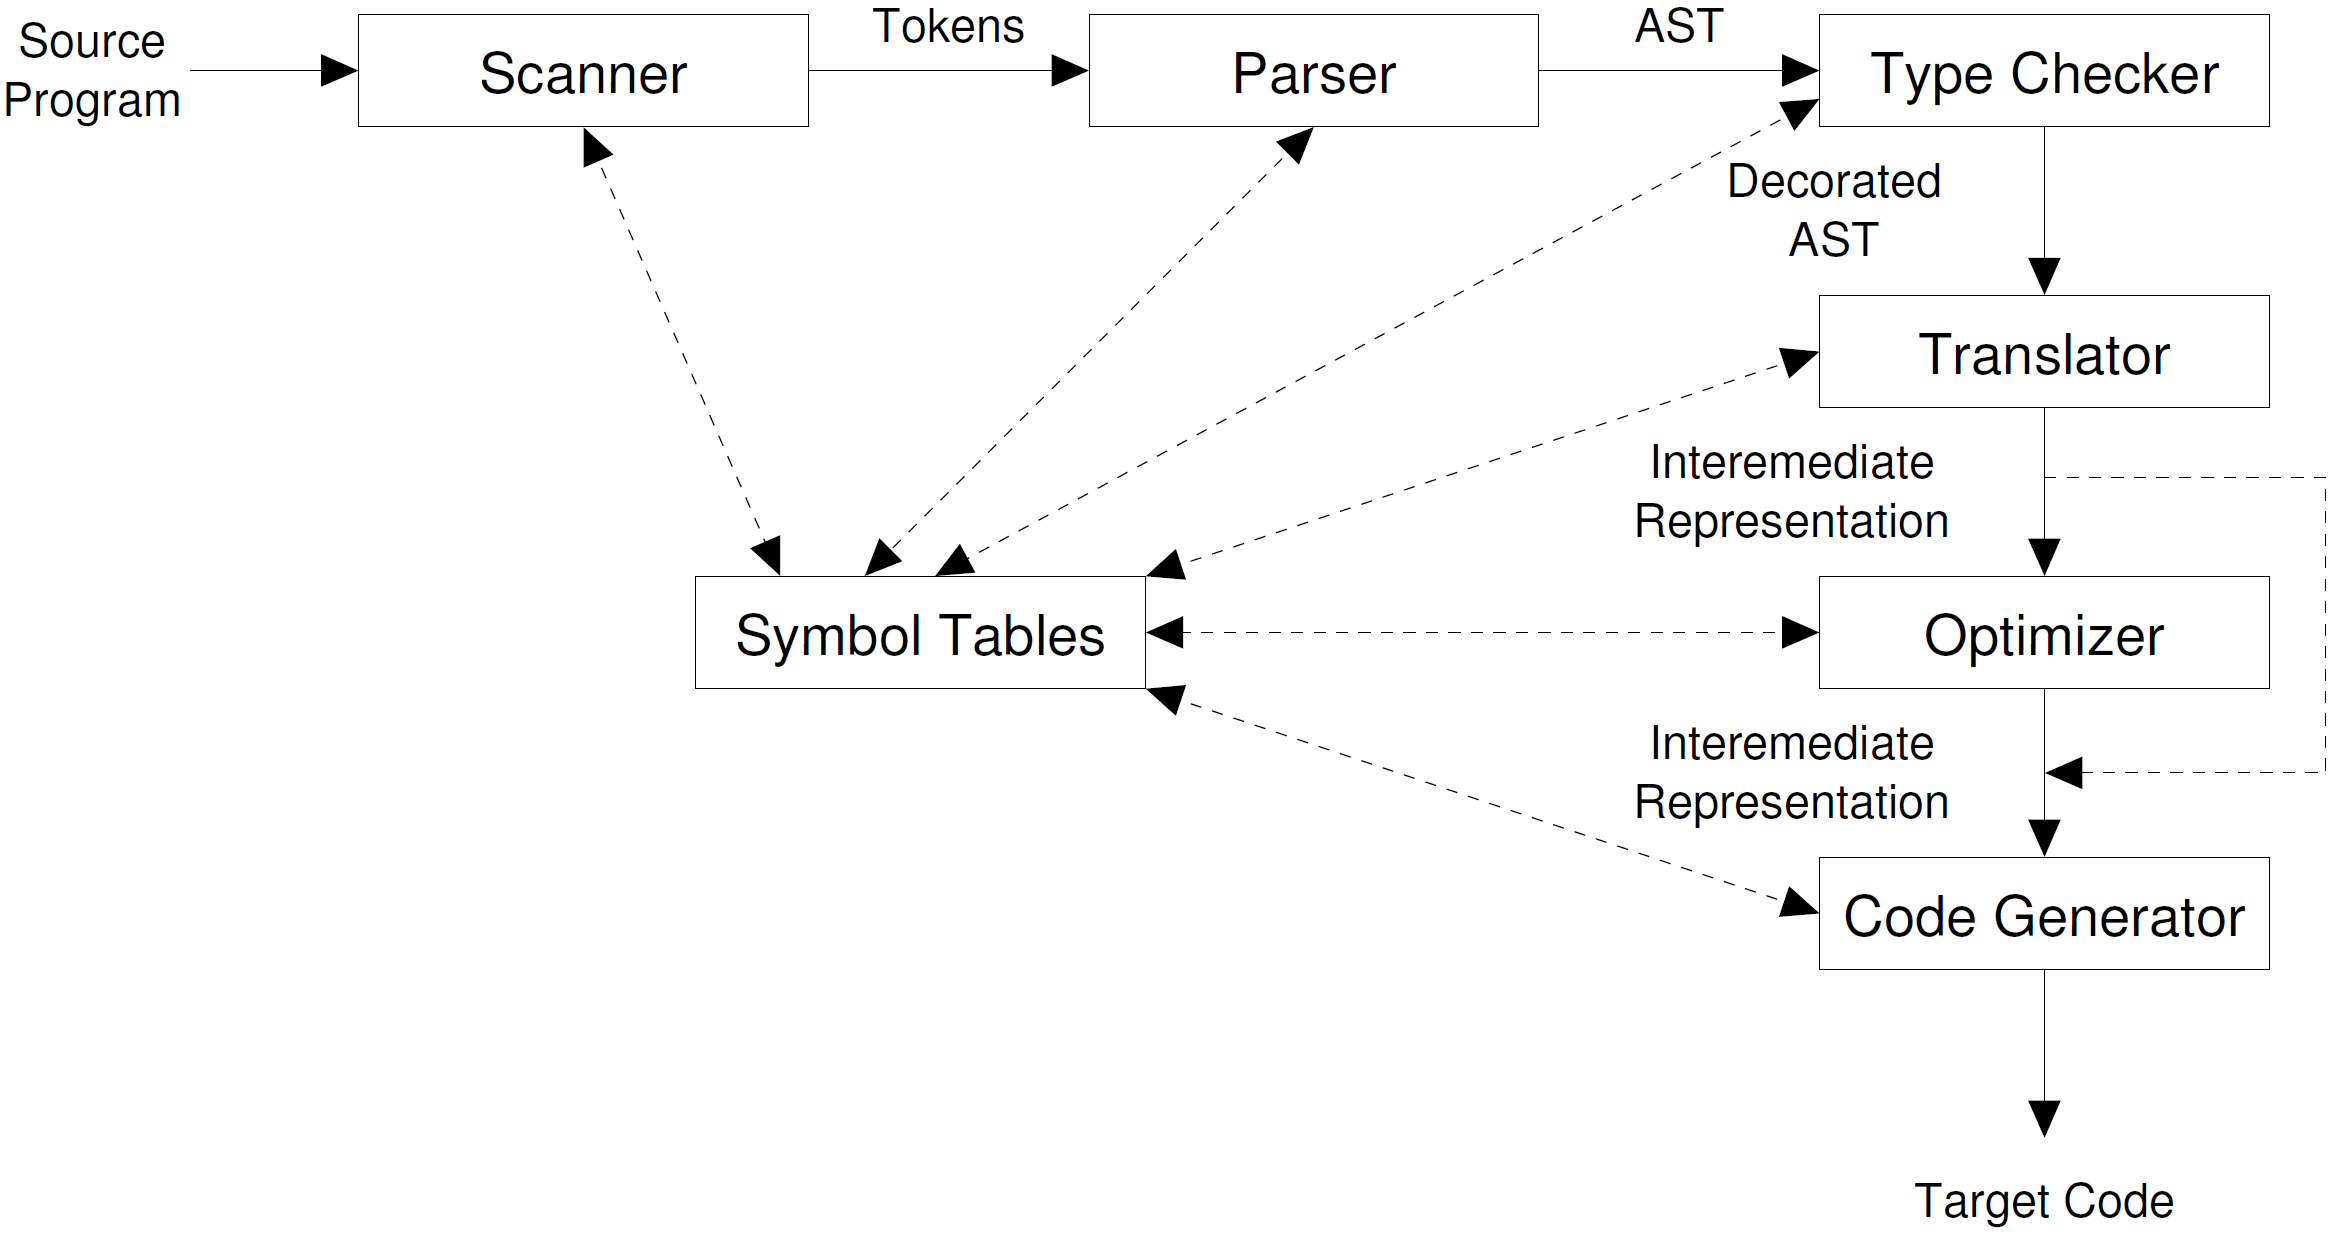
\includegraphics[width=0.8\textwidth]{figures/Full_Compiler.png}
    \caption{A textbook example of a compiler~\cite{CraftingCompiler}}
    \label{fig:generalcompilermodel}
\end{figure}


The target code is often low-level code for a particular system or runtime, but not always. When the target code is another high-level language, the process is also called transpilation. The Arc language is used for programming Arduinos, and so the compiler has to either generate Arduino-specific machine code or transpile it to the high-level Arduino language. Because the Arc language leverages the Protothreads library and its concurrency model for the Arduino, it makes sense for the Arc compiler to be a transpiler.

The Arc compiler follows many of the steps of the general model. Figure~\ref{fig:arccompilermodel} models the Arc compiler with some essential details.


\begin{figure}[htb!]
    \centering
    \begin{tikzpicture}[node distance=3cm]
        \begin{scope}[node distance=3cm,local bounding box=clusterA]
            \node (a) [state] {Scanner} node[below,scale=.7, xshift=60,yshift=-20]{Antlr};
            \node (b) [state, right of=a] {Parser};
            \draw[arrow, ->] (a) -- node[above,scale=.70,align=center]{Tokens} (b);
        \end{scope}

        \node(clusterA_g)[cluster,fit=(clusterA)]{};
        \node (start) [shift={($(clusterA.west)+(-2cm,0)$)}] {Source code};
        \node (c) [state, right of = b] {Type checker};
        \node (d) [state, shift={($(c.south)+(0,-1.5cm)$)}] {Scope checker};
        \node (e) [state, shift={($(d.south)+(0,-1.5cm)$)}] {Code generator};
        \node (f) [shift={($(e.south)+(0,-1cm)$)}] {Target code};

        \draw[arrow, ->] (start) -- (clusterA_g);
        \draw[arrow, ->] (b) -- node[right,scale=.70,xshift=-10,yshift=7]{AST} (c);
        \draw[arrow, ->] (c) -- node[right,scale=.70,align=center]{AST} (d);
        \draw[arrow, ->] (d) -- node[right,scale=.70,align=center]{AST} (e);
        \draw[arrow, ->] (e) --  (f);

    \end{tikzpicture}
    \caption{The Arc compiler model.}
    \label{fig:arccompilermodel}
\end{figure}


Figure~\ref{fig:arccompilermodel} shows how the source code is first scanned into tokens and then parsed into an \gls{ast}. \gls{antlr} generates the lexer and parser for this from our grammar, hence the box around the scanner and parser. The \gls{ast} is then type-checked and scope-checked. The type and scope check rules are explained in more detail in section\ref{sec:contextualconstraints}. Once the transpiler has done all of the necessary checks on the source code, it is ready to generate the Arduino code, which is also the final step of the compiler. We now have target code ready for the Arduino based on our source Arc code.